\documentclass[12pt]{article}
	
\title{CSC 320 - Worksheet 3}
\author{Nadeem Abdul Hamid}
\date{January 18, 2024}  


\usepackage[margin=1in]{geometry}		% For setting margins
\usepackage{amsmath}				% For Math
\usepackage{amsthm}
\usepackage{fancyhdr}				% For fancy header/footer
\usepackage{graphicx}				% For including figure/image
\usepackage{cancel}					% To use the slash to cancel out stuff in work
\usepackage[shortlabels]{enumitem}
\usepackage{hyperref}
\usepackage{jigsaw}

\usepackage{algorithm,caption}
\usepackage{algpseudocodex}
% docs: https://ctan.math.washington.edu/tex-archive/macros/latex/contrib/algpseudocodex/algpseudocodex.pdf


%%%%%%%%%%%%%%%%%%%%%%
% Set up fancy header/footer
% taken from https://www.overleaf.com/latex/templates/homework-template/yvgnmrbywwnp
\makeatletter    % for \@ in \@title
\pagestyle{fancy}
\fancyhead[LO,L]{\@author}
\fancyhead[CO,C]{\@title}
\fancyhead[RO,R]{\@date}
\fancyfoot[LO,L]{}
\fancyfoot[CO,C]{\thepage}
\fancyfoot[RO,R]{}
\renewcommand{\headrulewidth}{0.4pt}
\renewcommand{\footrulewidth}{0.4pt}
\makeatother    % restore
%%%%%%%%%%%%%%%%%%%%%%


%%%%%%%%%%%%%%%%%%%%%%
% from: https://tex.stackexchange.com/questions/14667/does-latex-define-a-semantic-equivalent-of-textbf
\makeatletter
\newcommand{\strong}[1]{\@strong{#1}}
\newcommand{\@@strong}[1]{\textbf{\let\@strong\@@@strong#1}}
\newcommand{\@@@strong}[1]{\textnormal{\let\@strong\@@strong#1}}
\let\@strong\@@strong
\makeatother
%%%%%%%%%%%%%%%%%%%%%%


\newcommand{\emptybox}[2][\textwidth]{%
  \begingroup
  \setlength{\fboxsep}{-\fboxrule}%
  \noindent\framebox[#1]{\rule{0pt}{#2}}%
  \endgroup
}

\newtheorem{theorem}{Theorem}
\newtheorem{lemma}{Lemma}


\begin{document}

\section{Recurrence relations; Analysis of recursive algorithms}

\subsection{Recurrence relations}

Solve the following recurrence relations.\\~

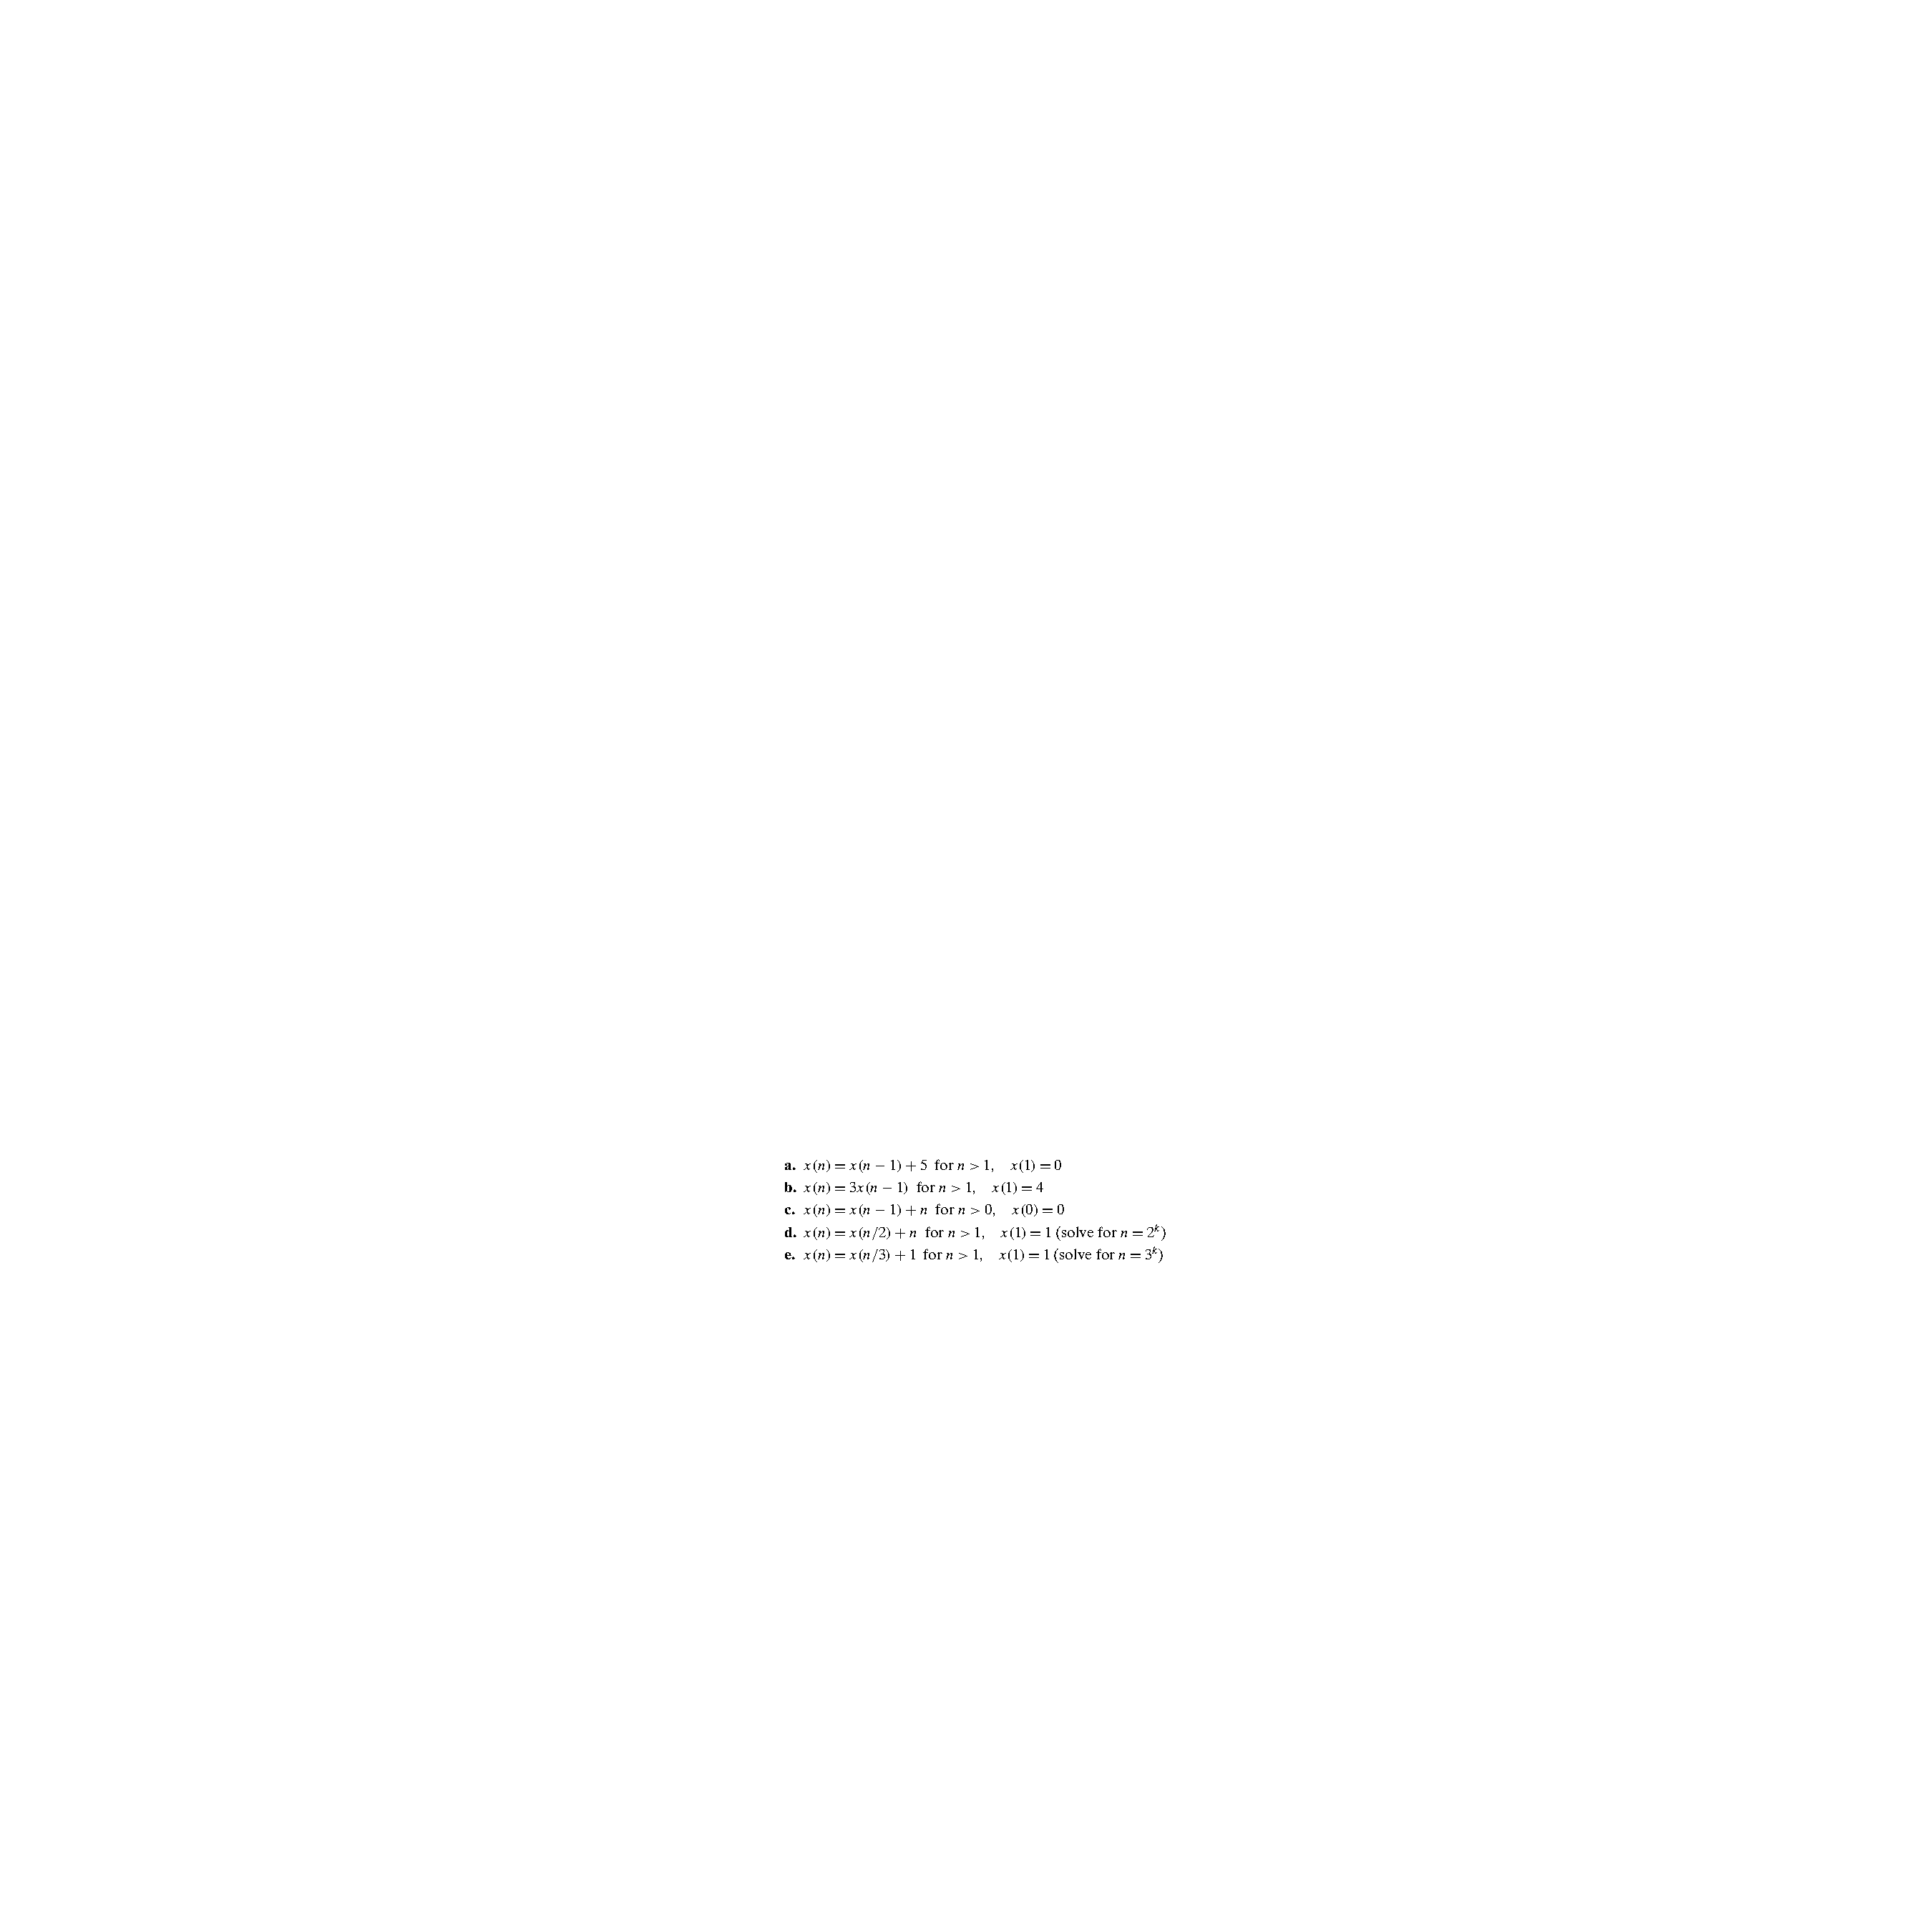
\includegraphics{w03-recs.pdf}


\clearpage
\subsection{Recursive algorithm}

Consider the following recursive algorithm for computing the sum of the first $n$ cubes:\\ $S(n) = 1^3 + 2^3 + \dots + n^3$.\\ ~

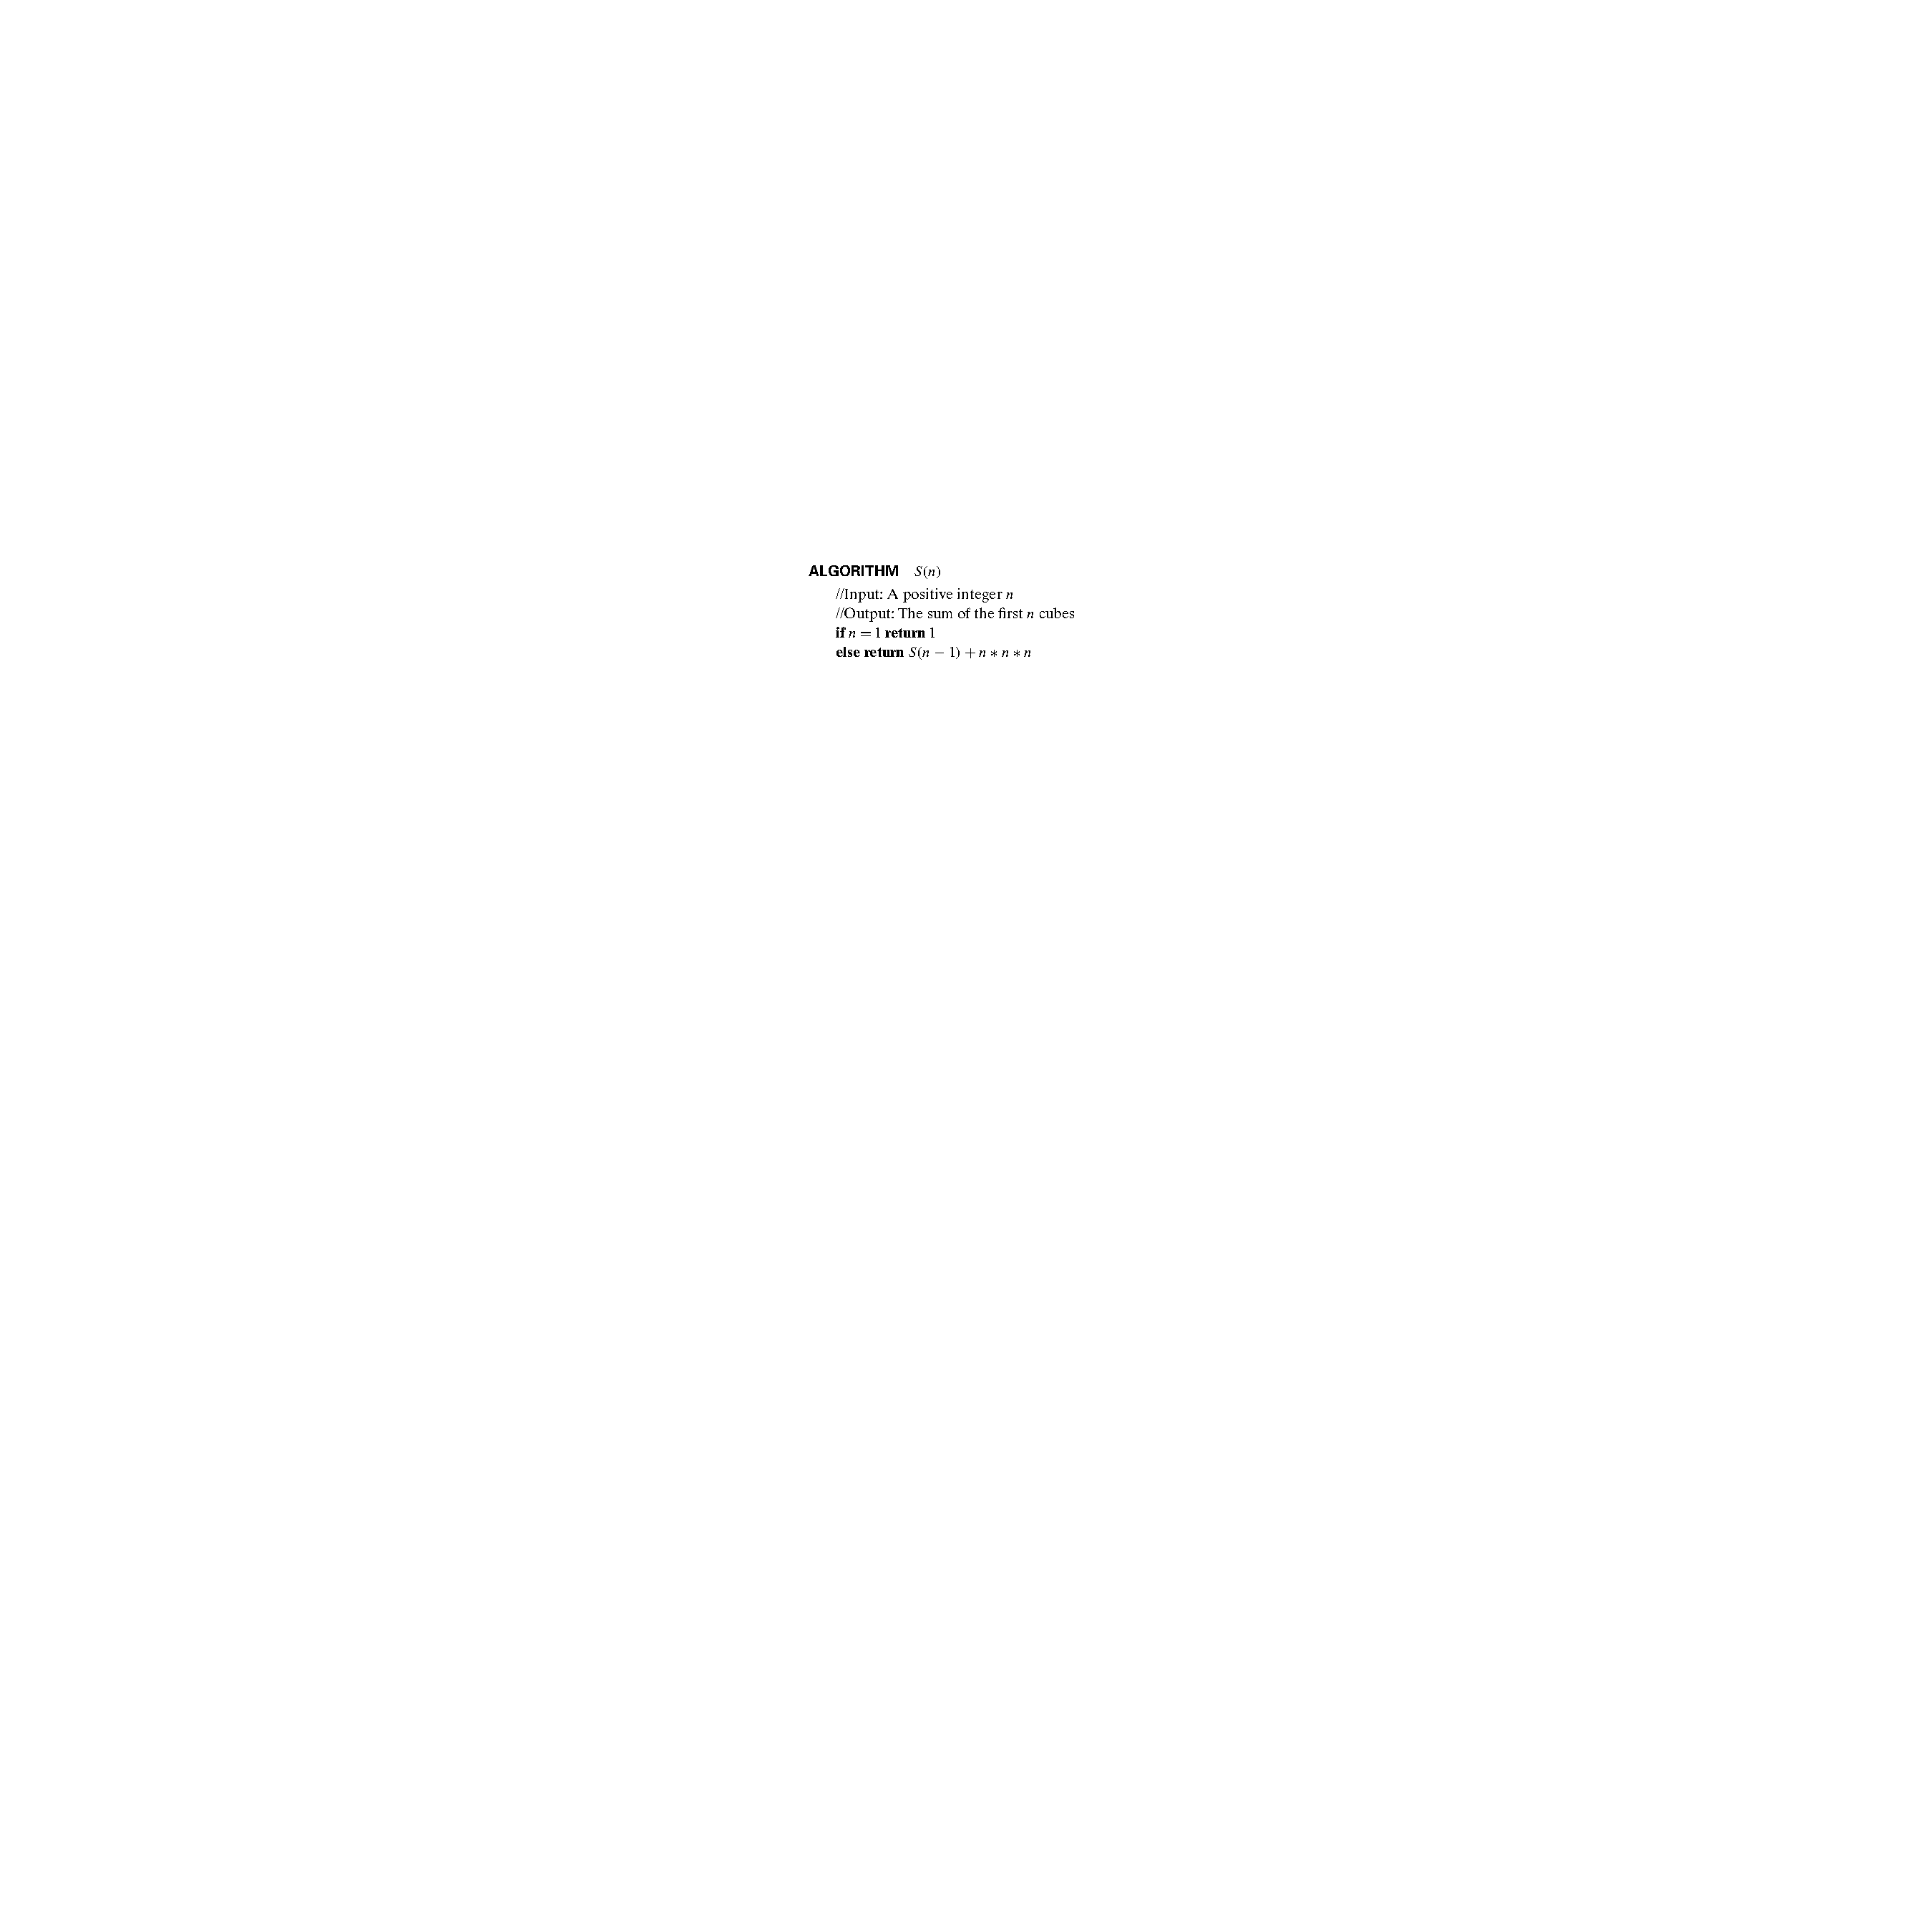
\includegraphics{w03-alg-S.pdf}

\begin{enumerate}[a.]
    \item Set up and solve a recurrence relation for the number of times the algorithm's basic operation is executed.
    \item How does this algorithm compare with the straightforward nonrecursive algorithm for computing this sum?
\end{enumerate}



\clearpage
\subsection{Another recursive algorithm}

Consider the following recursive algorithm.\\~

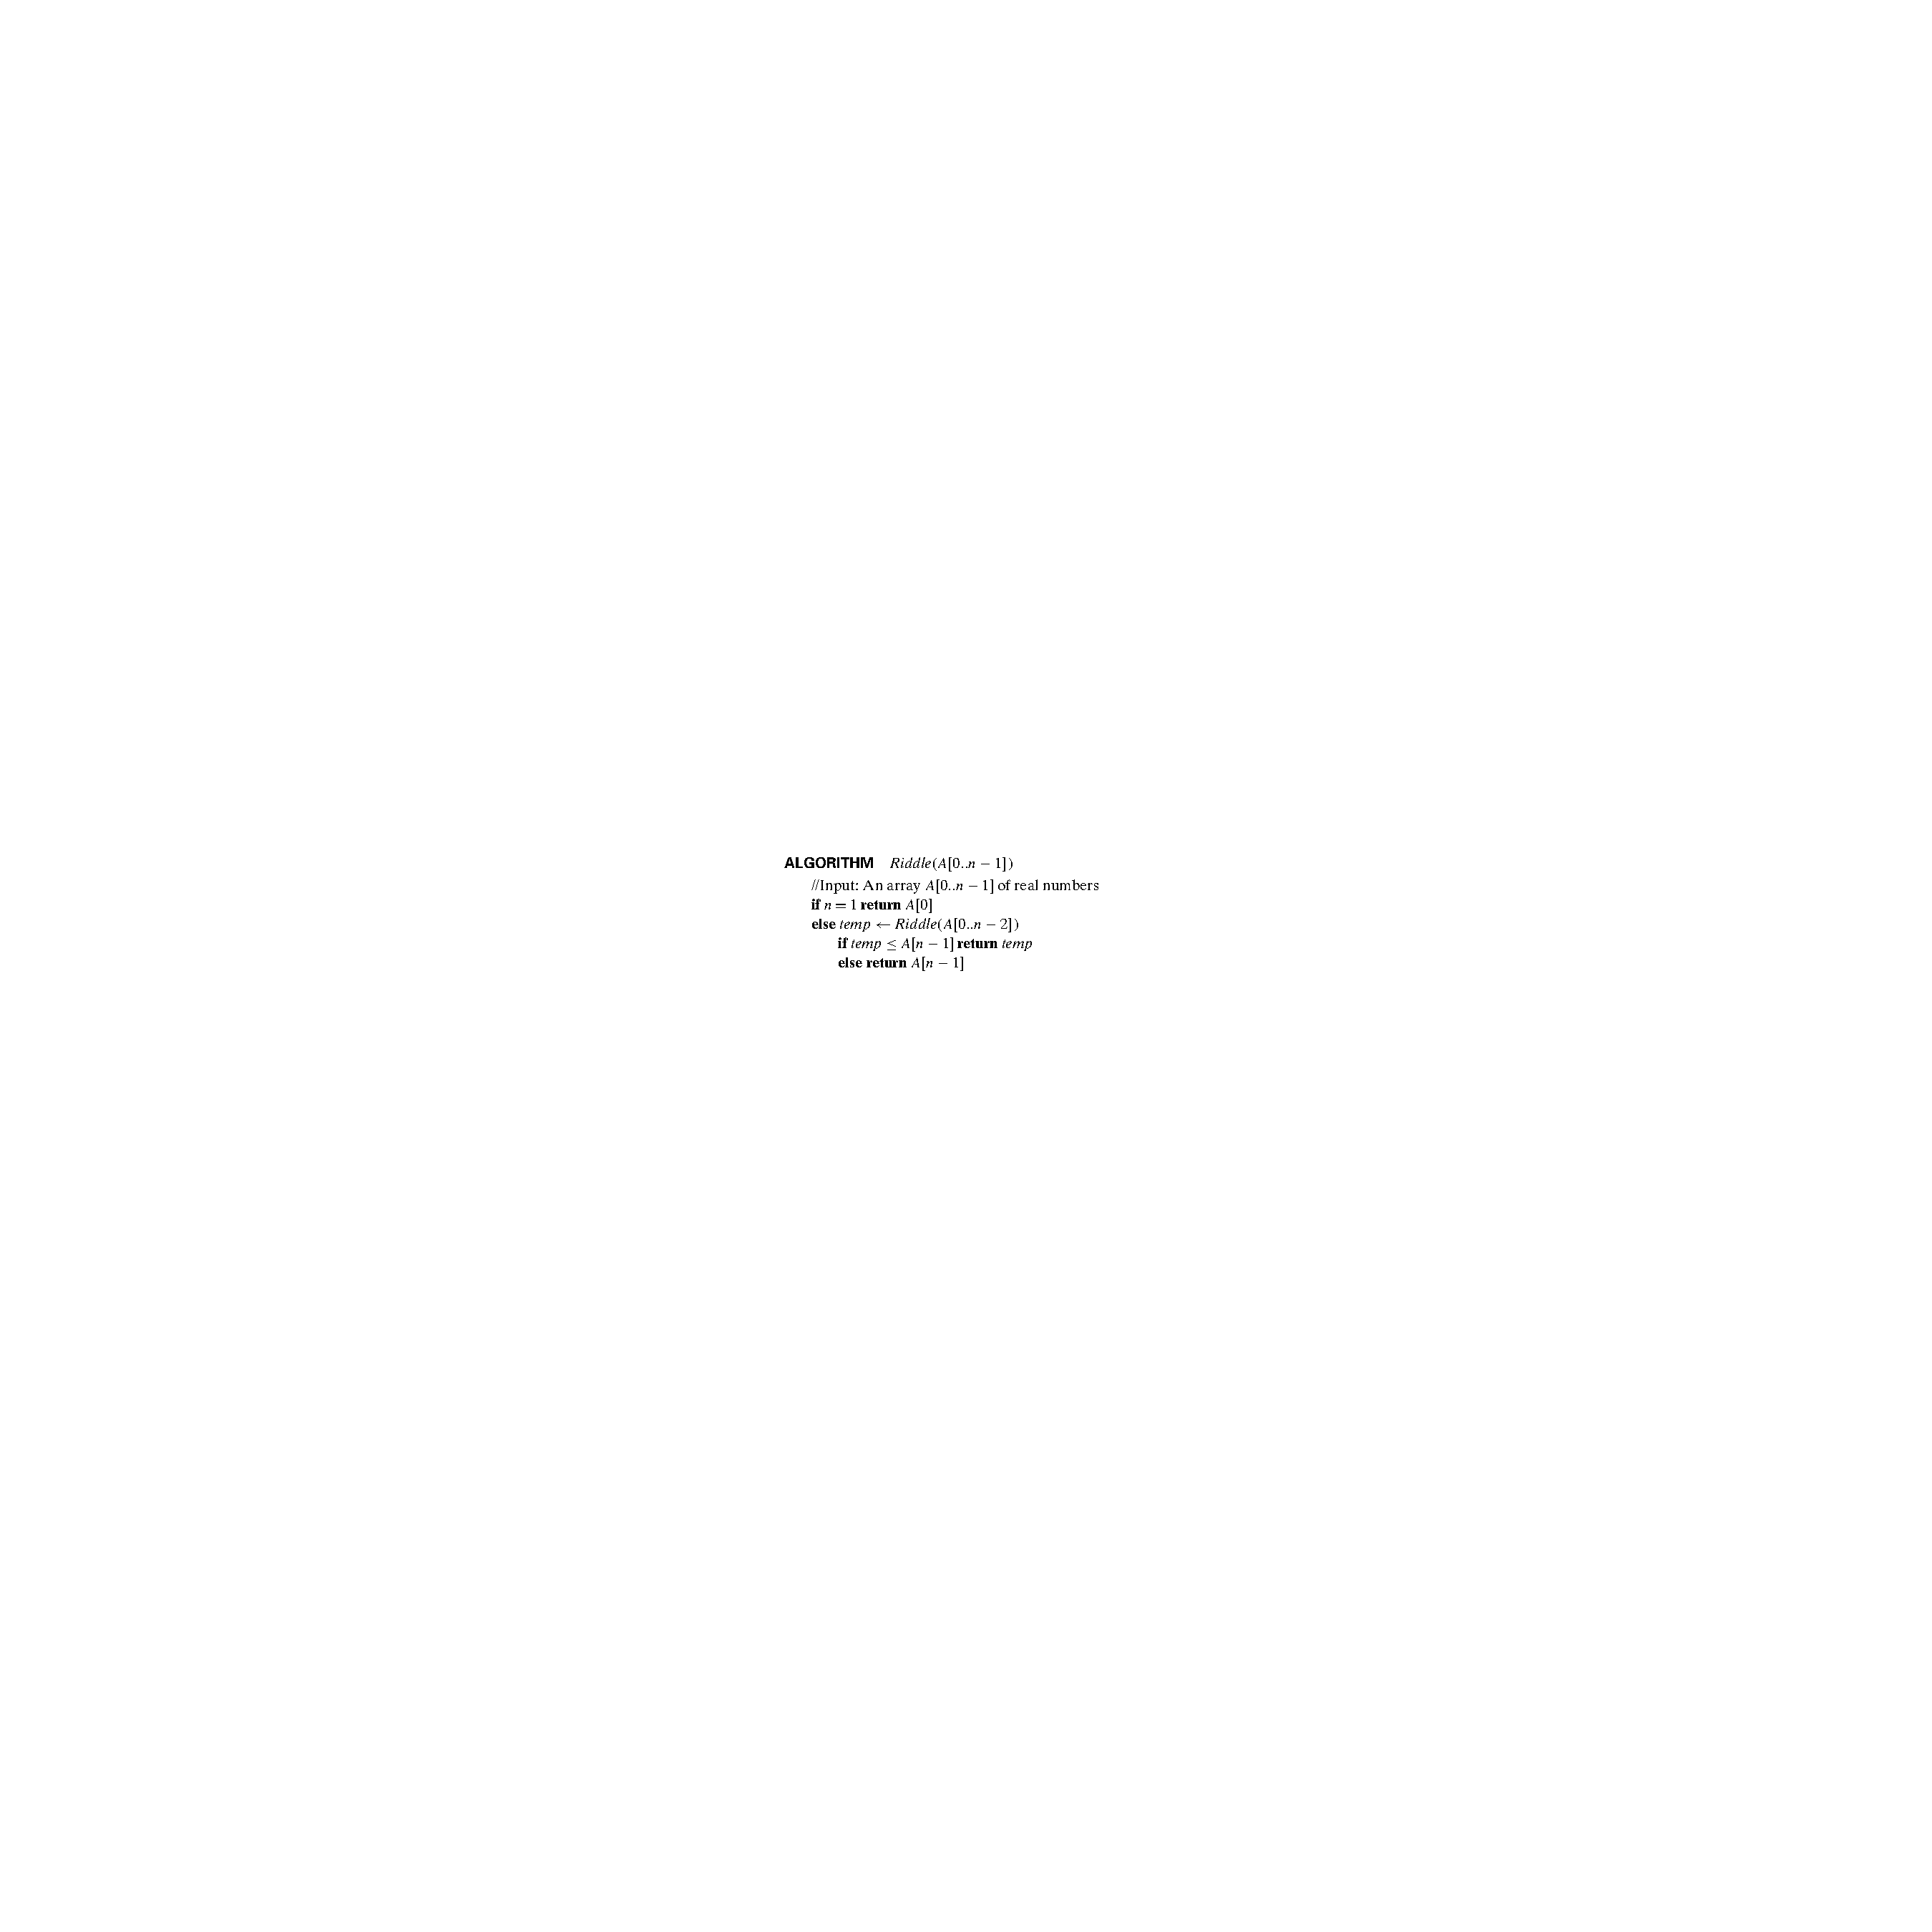
\includegraphics{w03-alg-riddle.pdf}

\begin{enumerate}[a.]
    \item What does this algorithm compute?
    \item Set up a recurrence relation for the algorithm's basic operation count and
    solve it.
\end{enumerate}



\end{document}



